\section{Ransac mit Maskierung} \label{sec:maskenbau}

Der nun folgend beschriebene Ansatz zur Detektion der Fahrbahnlinien ist in der endgültigen Implementierung nicht zum Einsatz gekommen. Da wir uns jedoch lange Zeit damit beschäftigt und viele später weiter verwendete Grundfunktionen aufgebaut haben, wird die Vorgehensweise nun näher erläutert.

Die Implementierung begann bereits vor Fertigstellung der Hardware. Zu jenem Zeitpunkt ist deshalb der Bildausschnitt noch nicht so, wie in~\ref{fig:bildvorverarbeitung_entzerren} zu sehen, gewählt worden, weshalb die Abbildungen~\ref{fig:fahrspurerkennung_ransac_binarisieren}, ~\ref{fig:fahrspurerkennung_ransac_masken} und~\ref{fig:fahrspurerkennung_ransac_ransac} einen anderen Teilbereich darstellen. Das ändert indes nichts an dem Algorithmus selbst, sondern ist nur eine Sache der Parametereinstellungen. 

Nachdem das Foto binarisiert wurde, stellen alle Pixel mit dem Wert \glqq 1\grqq{} im Idealfall potenzielle Linienpunkte dar, die aber noch der richtigen Kategorie \glqq linke\grqq , \glqq mittlere\grqq{} oder \glqq rechte\grqq{} Linie zugeordnet werden müssen oder durch den \gls{acr:ransac}-Algorithmus als \gls{glos:outlier} markiert sind. Dazu muss eine \gls{acr:roi} festgelegt werden, also eine entsprechende Maske, die über das Bild gelegt wird. Die Idee war, die Maske so zu bauen, wie wir anhand unserer bereits eingetragenen Punkte in der Weltkarte und der Pose zum Zeitpunkt der Bildaufnahme die zur Linie zugehörigen Pixel erwarten konnten. Die Weltkarte ist ein Struktur-Feld, in dem unter anderem die Koordinaten der eingetragenen Linienpunkte gespeichert sind, jedoch nicht deren approximierte Funktion. Zur Gewinnung der entsprechenden \gls{acr:roi} wird ein Fit der Kartenpunkte in das Bild transformiert. Nach einer Dilatation der im Bildausschnitt liegenden Funktion um einen Parameterwert entsteht ein dickes Band von Punkten, die die \gls{acr:roi} bilden (siehe Abbildung~\ref{fig:fahrspurerkennung_ransac_masken}).

% entzerrtes und binarisiertes Beispielbild und Filterergebnisse für Mittellinie nebeneinander (4 Bilder)
\begin{figure}[H]
  \centering
  \subfloat[][]{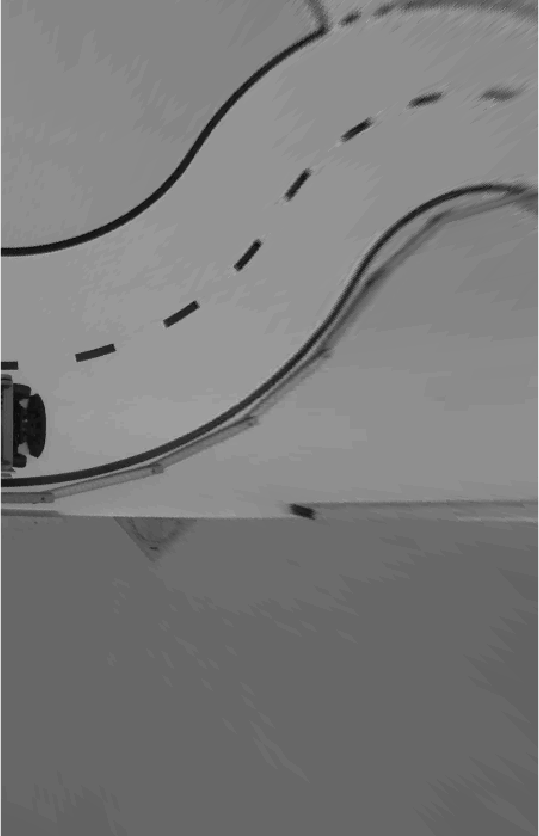
\includegraphics[width=0.35\textwidth]{fahrspurerkennung_ransac_imgUndist.png}}
  \qquad \quad
  \subfloat[][]{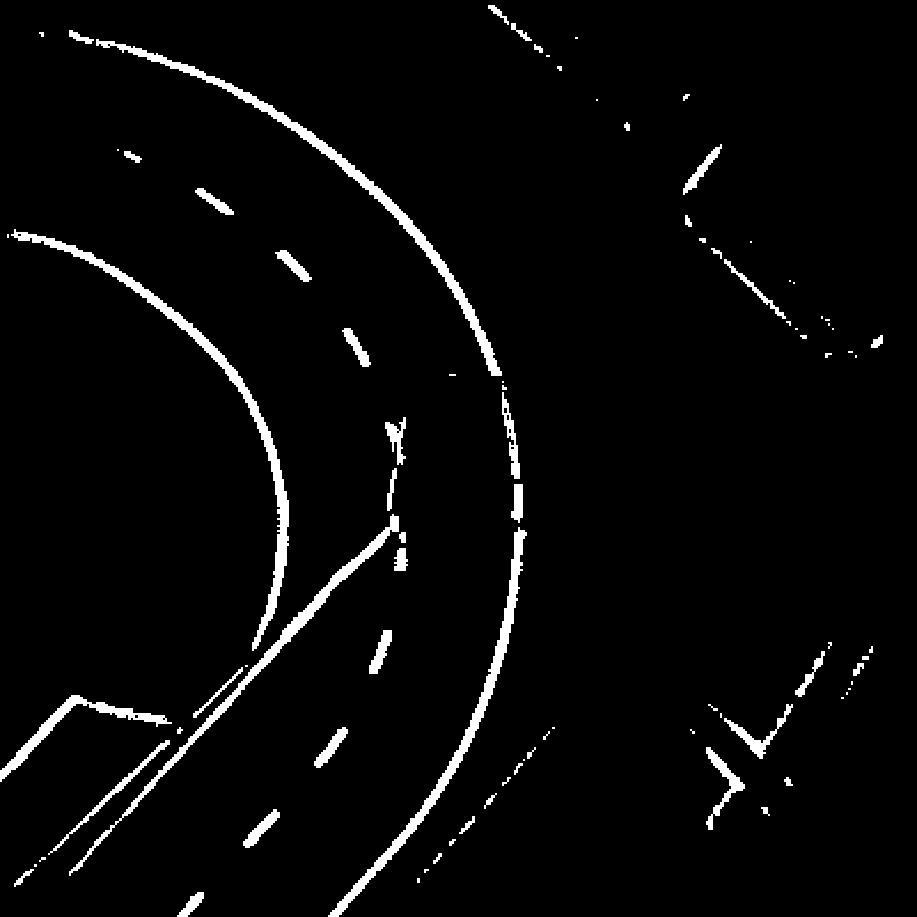
\includegraphics[width=0.35\textwidth]{fahrspurerkennung_ransac_imgBinarized.png}}
  \qquad \quad
  \subfloat[][]{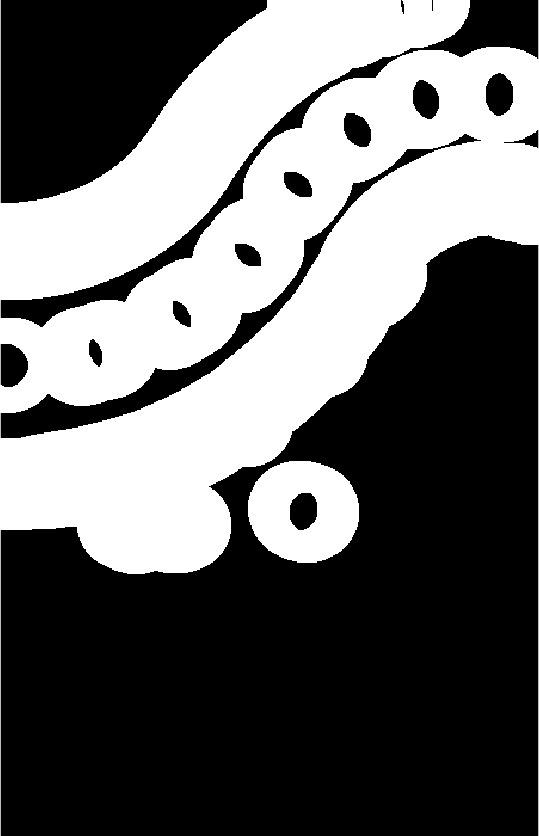
\includegraphics[width=0.35\textwidth]{fahrspurerkennung_ransac_imgMidFiltered.png}}
  \qquad \quad
  \subfloat[][]{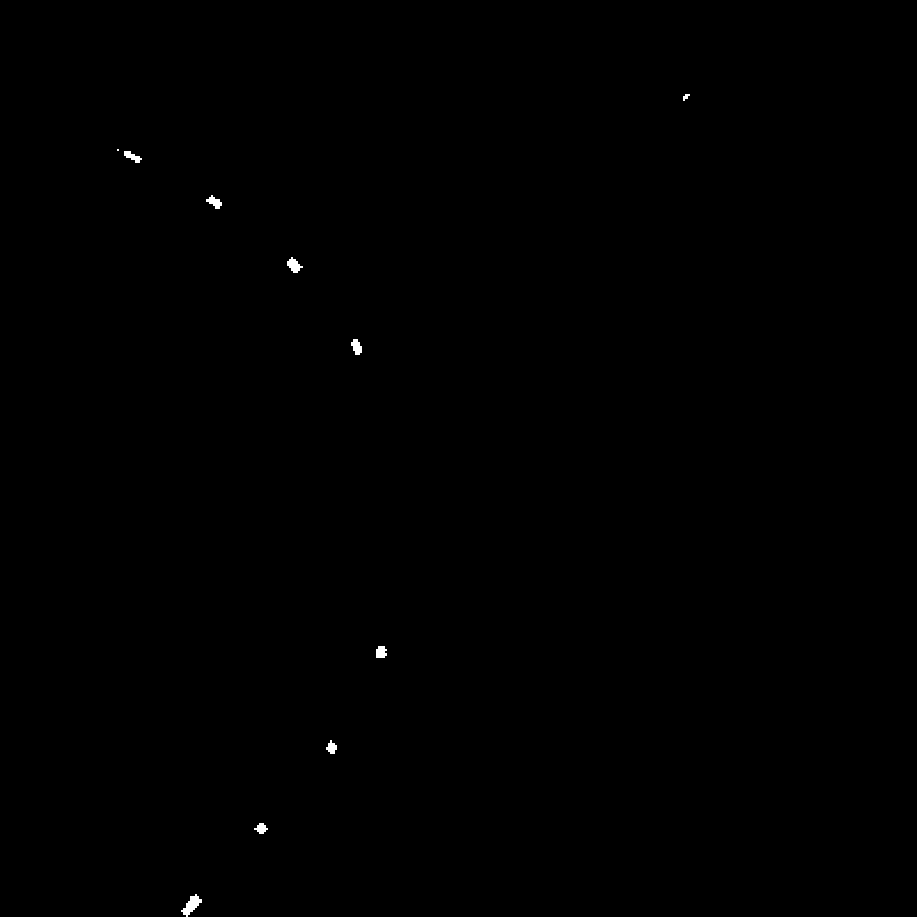
\includegraphics[width=0.35\textwidth]{fahrspurerkennung_ransac_imgBinarizedAndNotImgMidFiltered.png}}
  \caption{entzerrtes (a) und binarisiertes Bild (b) einer Testaufnahme auf der Strecke in alten Kameraeinstellungen; Filterergebnis des ''Ringfilters'' (c) und Durchschnitt dessen Negation mit dem binarisierten Bild (d)}
\label{fig:fahrspurerkennung_ransac_binarisieren}
\end{figure} 

% Textumflossenes Bild des ''Ringfilter''-Kerns
\begin{wrapfigure}{r}{0.5\textwidth}
 \centering
  
\includegraphics[width=0.3\textwidth]{fahrspurerkennung_ransac_midfilter.png}
  \caption{Der Kern des \\ \glqq Ringfilters\grqq}
\label{fig:fahrspurerkennung_ransac_midfilter}
\end{wrapfigure} 

\paragraph{Initialer Maskenbau} 

Ein nicht zu vernachlässigendes Problem stellt allerdings noch die Initialisierung dar. Wie baut man die Masken, wenn noch keine Linienpunkte in die Karte eingetragen worden sind? Die einfachste und am Anfang auch implementierte Möglichkeit bietet die hart aus Parameterwerten vorgeschriebene Maske einer Gerade, in der Annahme, das Auto starte immer auf einem geraden Abschnitt. Da so die Robustheit aber schlecht gewährleistet ist, wurde dies schnell wieder verworfen und eine bessere Möglichkeit gefunden. Die gestrichelte Mittellinie besitzt im ganzen Bild Alleinstellungsmerkmale, die sich durch ein darauf angepasstes weiteres Faltungsfilter nutzen lassen. Den in Abbildung~\ref{fig:fahrspurerkennung_ransac_midfilter} gezeigten Filterkern haben wir \glqq Ringfilter\grqq{} genannt (Idee entnommen aus \autocite{drauschkeEchtzeitfaehigeStartpunktalgorithmenFuer2016}). Er ist aus einem Innen- und Außenkreis entworfen, sodass der Radius des inneren Kreises mindestens so groß wie die Länge eines Mittellinienstriches im Bild und der Außenkreisradius maximal so groß wie der kürzeste Abstand zwischen zwei Mittellinienstrichen ist. Was als Filterergebnis beispielhaft herauskommt, ist in (c) der Abbildung~\ref{fig:fahrspurerkennung_ransac_binarisieren} zu erkennen. Das Filter bewirkt, dass im Ergebnisbild genau dann ein Pixel mit \glqq 1\grqq{} beschrieben wird, wenn der Filterring um dieses Pixel mindestens einen Punkt im binarisierten Bild schneidet. Es entstehen also \glqq schwarze Flecke\grqq{} an den Stellen, wo Mittellinienstriche innerhalb des \glqq Ringfilters\grqq{} liegen. Die Negation des Filterergebnisses als Maske auf das binarisierte Bild gelegt erzeugt eine Grafik, die allein Pixel aus Punktgruppen enthält, die eine festgelegte Maximallänge und einen Mindestabstand zu anderen Punkten besitzen. Darauf kann nun der \gls{acr:ransac}-Algorithmus angewendet werden. Dass hier noch \gls{acr:ransac} sinnvoll und notwendig ist, sieht man in (d) von Abbildung~\ref{fig:fahrspurerkennung_ransac_binarisieren} an der weißen Pixelgruppe unten im Bild, die nicht zur mittleren Fahrbahnmarkierung gehört.

Die zwei initialen Masken für die Randlinien werden anschließend aus der approximierten Funktion dritten Grades der Mittellinie gebildet. Dies geschieht aus der gerichteten Verschiebung diskreter Punkte der Approximation. Gleichung~\ref{eq:polynom3} sei eine mathematische Beschreibung der Funktion, die den Linienverlauf approximiert, dann ist Gleichung~\ref{eq:derr_polynom3} die Ableitung, welche den Anstieg an den Stellen \( x \) beschreibt. Der Verschiebungsvektor \( \boldsymbol{r} \) steht dann senkrecht auf \gls{lat:func}.

\begin{eqnarray}
\gls{lat:func}(\gls{lat:xcoord}) & = & ax^3 + bx^2 +cx +d  \label{eq:polynom3} 	\\
f’(x) & = & 3ax^2 + 2bx +c \label{eq:derr_polynom3} 							\\
\boldsymbol{r} & = & \frac{1}{\sqrt{(-f’(x))^2 + 1}} \cdot
\begin{pmatrix}
-f’(x) 	\\
1 		\\
\end{pmatrix}
\label{eq:maske_verschiebungsvektor}									\\
\begin{pmatrix}
x_s 	\\
y_s	\\
\end{pmatrix}
 & = & 
 \begin{pmatrix}
x 	\\
y	\\
\end{pmatrix}
\pm l \cdot \boldsymbol{r}  
\label{eq:maske_randpunkte}
\end{eqnarray}

Die Normierung von \( \boldsymbol{r} \) multipliziert mit der bekannten Fahrspurbreite \( l \) addiert auf den Mittellininenpunkt \( (x,y)^T \) ergibt einen Stützpunkt \( (x_s,y_s)^T \) der linken (\( + \)) bzw. der rechten (\( - \)) Randlinie (Gleichungen~\ref{eq:maske_verschiebungsvektor} und~\ref{eq:maske_randpunkte}).

Durch die so verschobenen Stützpunkte der erwarteten Lage der Randlinien werden ein neuer Fit und eine anschließende Dilatation vorgenommen, um die initialen Randmasken zu erzeugen. Um auszuschließen, dass man zur mittleren Strichlinie zugehörige Bildpunkte einer Randlinie zuordnet, wird zusätzlich eine elementweise UND-Operation mit der negierten Mittellinienmaske durchgeführt. Die verhinderte Überschneidung der Masken ist auch in Abbildung~\ref{fig:fahrspurerkennung_ransac_masken} zu erkennen.

% Bilder der drei Masken für linke, mittlere und rechte Linie
\begin{figure}[H]
  \centering
  \subfloat[][]{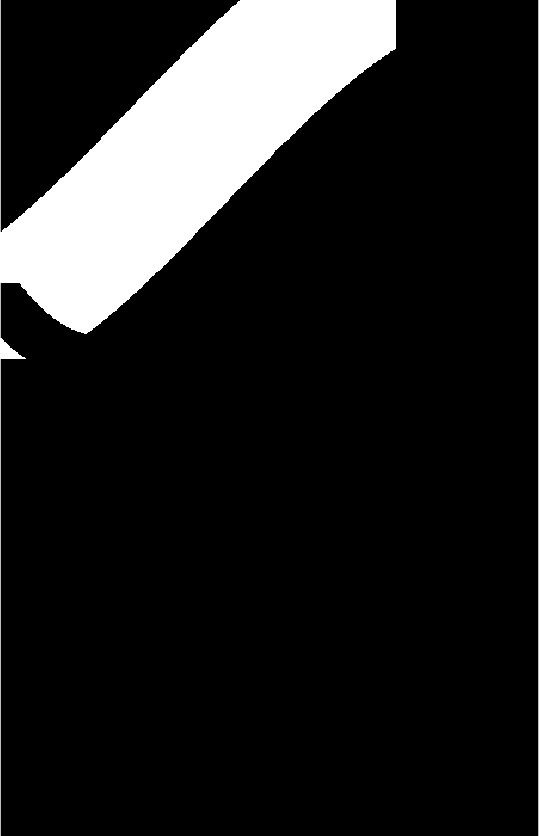
\includegraphics[width=0.3\textwidth]{fahrspurerkennung_ransac_imgMaskLeft.png}}
  \quad
  \subfloat[][]{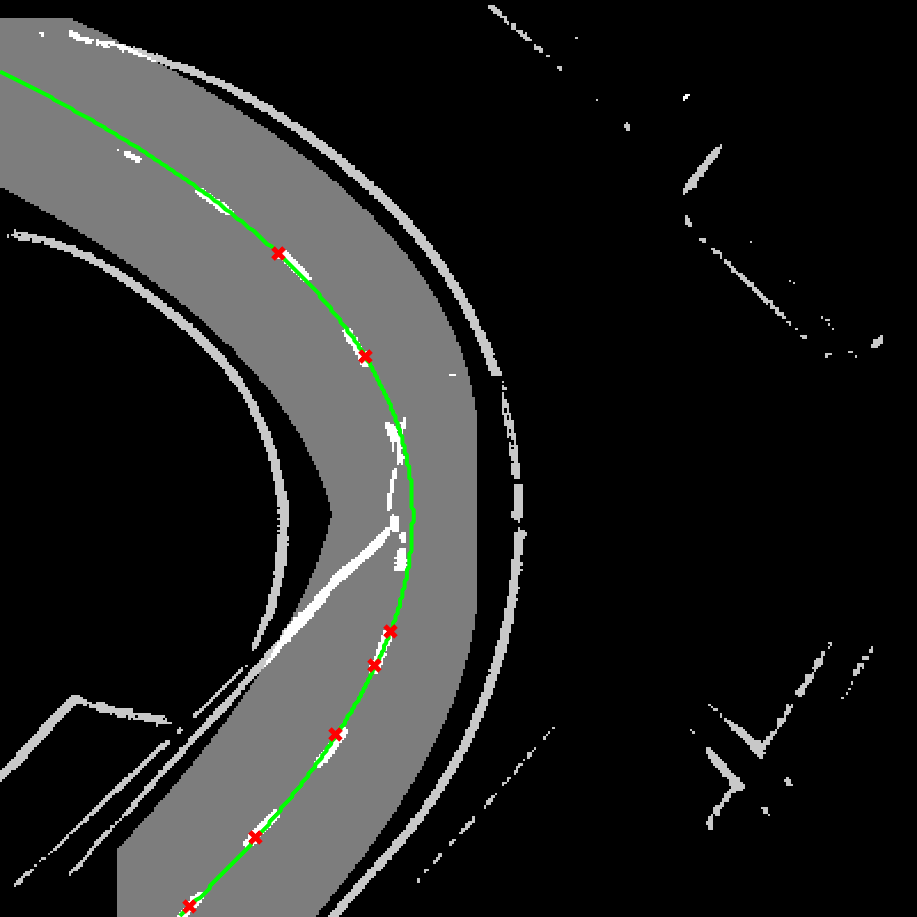
\includegraphics[width=0.3\textwidth]{fahrspurerkennung_ransac_imgMaskMiddle.png}}
  \quad
  \subfloat[][]{
\includegraphics[width=0.3\textwidth]{fahrspurerkennung_ransac_imgMaskRight.png}}
  \caption{Masken zum Herausschneiden der linken (a), mittleren (b) und rechten (c) Fahrbahnmarkierung für die Anwendung des \gls{acr:ransac}-Algorithmus}
\label{fig:fahrspurerkennung_ransac_masken}
\end{figure} 

% Bilder der drei Ausführungen des RANSAC für linke, mittlere und rechte Linie
\begin{figure}[H]
  \centering
  \subfloat[][]{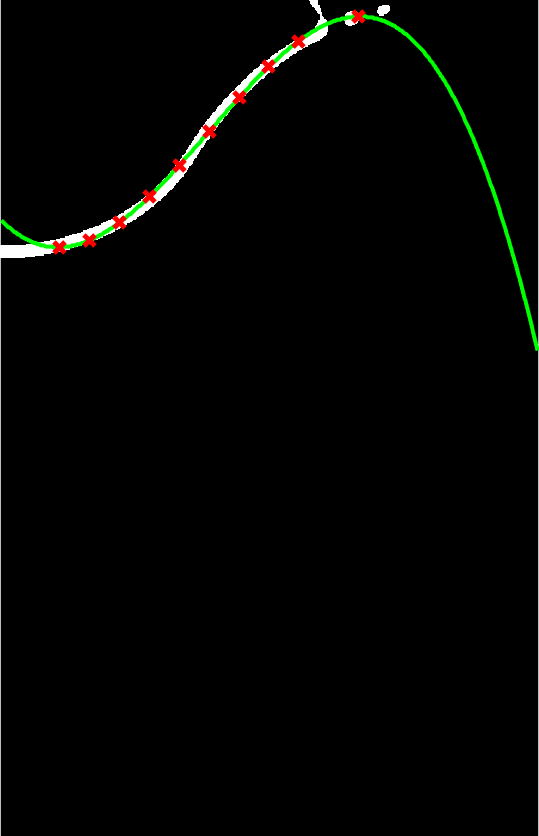
\includegraphics[width=0.3\textwidth]{fahrspurerkennung_ransac_imgRansacLeft.png}}
  \quad
  \subfloat[][]{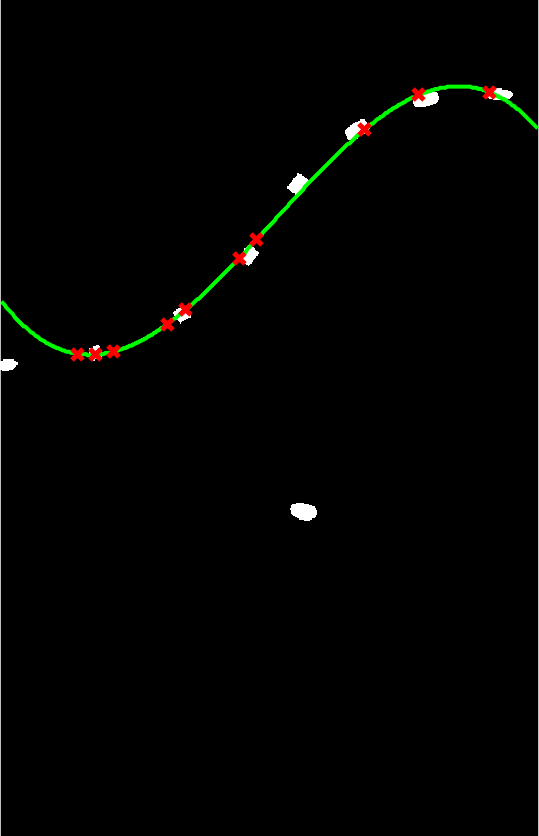
\includegraphics[width=0.3\textwidth]{fahrspurerkennung_ransac_imgRansacMiddle.png}}
  \quad
  \subfloat[][]{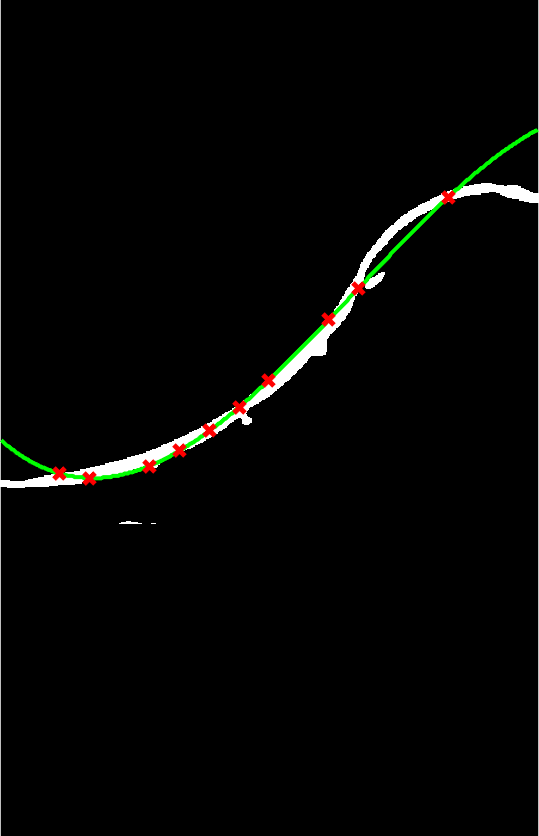
\includegraphics[width=0.3\textwidth]{fahrspurerkennung_ransac_imgRansacRight.png}}
  \caption{Approximation der linken (a), mittleren (b) und rechten (c) Fahrbahnmarkierungen durch eine Funktion dritten Grades mittels \gls{acr:ransac}}
\label{fig:fahrspurerkennung_ransac_ransac}
\end{figure} 

\paragraph{\gls{acr:ransac} und Weltkarte} 
Wie in Abbildung~\ref{fig:fahrspurerkennung_ransac_ransac} zu sehen, approximiert der \gls{acr:ransac}-Algorithmus den Verlauf der Fahrbahnlinien relativ gut. Die eingezeichnete grüne Funktion beschreibt das Ergebnis eines Fittes eines Polynoms dritten Grades durch die \gls{glos:inlier}. In einem bestimmten Abstand werden auf dem Polynom potentielle Kartenpunkte diskretisiert. Später werden in die Karte nur die Punkte eingetragen, welche sowohl auf der Funktion liegen als auch mit weißen Pixeln des maskierten Bildes übereinstimmen. So verhindern wir, Punkte an unpassenden Stellen in die Weltkarte einzutragen. Sie sind im Plot als Kreuze dargestellt. 

% Bild/Plot der eingetragenen Punkte in der Weltkarte
\begin{figure}[H] % [htb]
  \centering
  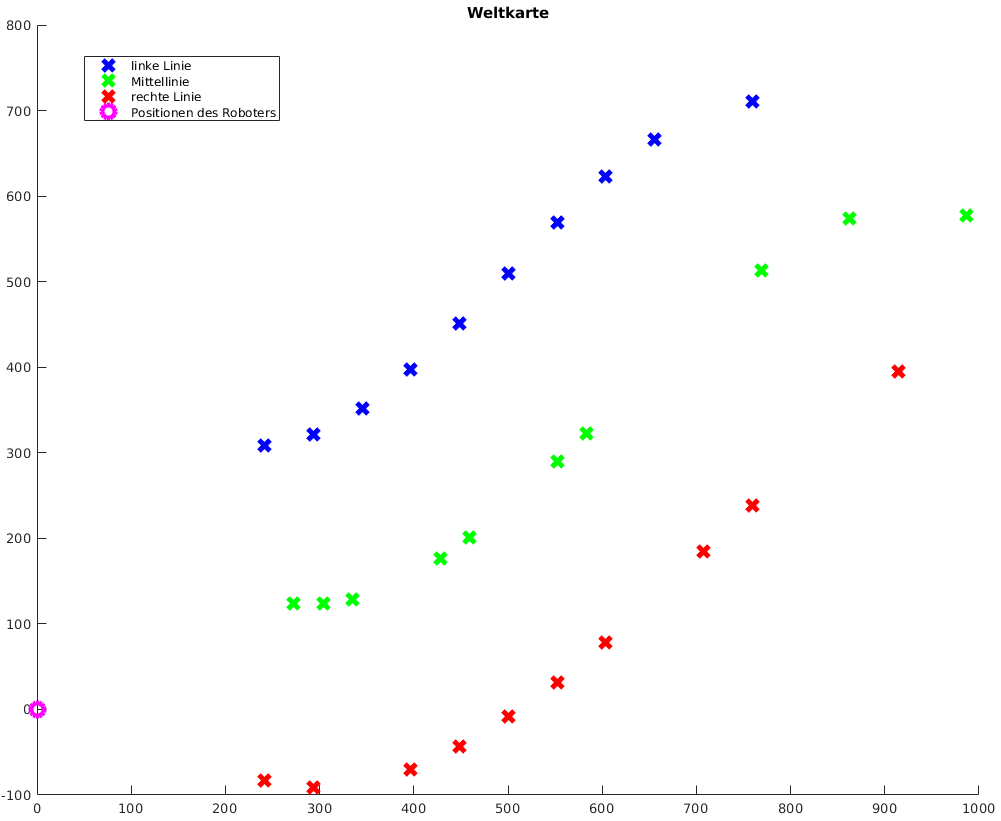
\includegraphics[width=0.9\textwidth]{fahrspurerkennung_ransac_plotWorldMap.png}
  \caption{Plot der eingetragenen Punkte in die Weltkarte}
\label{fig:fahrspurerkennung_ransac_karte}
\end{figure} 

